\section{Results}

\begin{figure}[t]
\centering
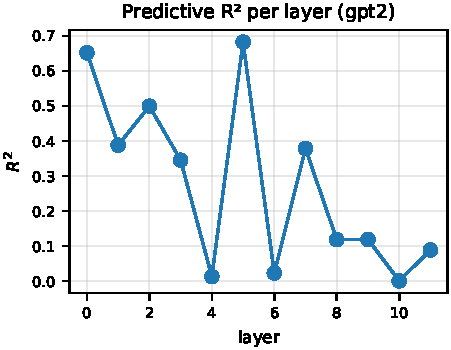
\includegraphics[width=\columnwidth]{figures/r2_per_layer_gptTwo.pdf}
\caption{Per-layer $R^2$ of mean attention entropy regressed on
compression ratio. The relationship peaks in the middle of the network
($R^2 = \gptTwoMaxRsq$ at layer $\gptTwoMaxRsqLayer$) and decays
toward the unembedding.}
\label{fig:r2}
\end{figure}

\begin{figure}[t]
\centering
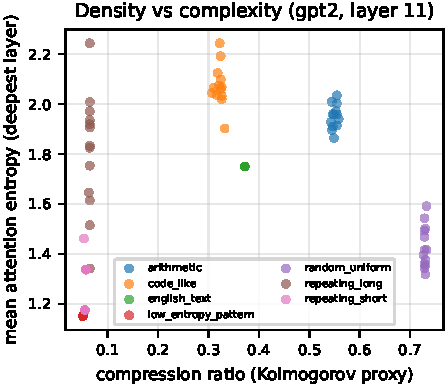
\includegraphics[width=\columnwidth]{figures/scatter_deep_gptTwo.pdf}
\caption{Scatter of mean attention entropy vs.\ compression ratio at
the deepest block. The $R^2$ is much lower
($\gptTwoDeepRsq$); families separate by horizontal position but
the within-family entropy distribution is broad.}
\label{fig:deep-scatter}
\end{figure}

\begin{figure}[t]
\centering
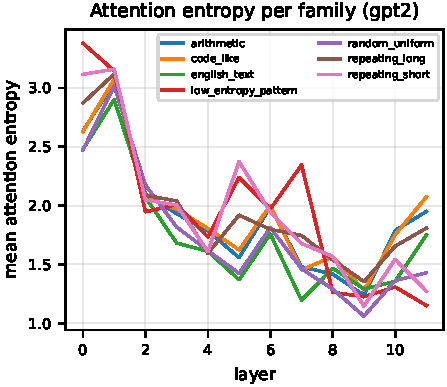
\includegraphics[width=\columnwidth]{figures/entropy_per_family_gptTwo.pdf}
\caption{Mean attention entropy by family and depth. Low-complexity
families (\textit{low\_entropy\_pattern}, \textit{repeating\_short})
sit clearly below the higher-complexity families through most of
the network, before re-converging near the head.}
\label{fig:entropy-family}
\end{figure}

\paragraph{Headline.}
At layer $\gptTwoMaxRsqLayer$, a univariate linear regression of
$\overline{H}_\ell$ on $\rho$ explains $\gptTwoMaxRsq$ of the
variance across the corpus. At the deepest layer, the same regression
gives $R^2=\gptTwoDeepRsq$ with slope $\gptTwoDeepSlope$.

\paragraph{Where the relationship lives.}
Figure~\ref{fig:r2} shows that the relationship is mid-network. We
interpret this as a Goldilocks zone: early layers attend on
syntactic patterns that depend less on global complexity; deep
layers compress information toward token logits, washing out the
prompt-level signal.
